\documentclass[10pt]{article}



\usepackage{amsmath}
\usepackage{amssymb}
\usepackage{amsthm}
\usepackage{array}
\usepackage{babelbib}
\usepackage{braket}
\usepackage{caption}
\usepackage{colortbl}
\usepackage{rotating}
\usepackage[table]{xcolor}
\usepackage{color}
\usepackage{enumerate}
\usepackage{esint}
\usepackage{eso-pic}
\usepackage{listings}
\usepackage{lscape}
\usepackage{mathtools}
\usepackage{multicol}
\usepackage{multirow}
\usepackage{physics}
\usepackage{siunitx}
\usepackage{subcaption}
\usepackage{subdepth}
\usepackage{tcolorbox}
\usepackage{tikz}
\usepackage{titlesec}
\usepackage{titling}
\usepackage{upgreek}
\usepackage{url}
\usepackage{verbatim}
\usepackage{vwcol}
\usepackage{wallpaper}
\usepackage{xfrac}
\usepackage[c]{esvect}
\usepackage[utf8]{inputenc}
\usepackage[fleqn]{nccmath}
\usepackage[thicklines]{cancel}
\usepackage[margin=2cm]{geometry}
\usepackage[colorlinks=true,spanish]{hyperref}
\usepackage[oldvoltagedirection]{circuitikz}
\usepackage[greek,spanish,es-tabla,es-nodecimaldot,es-noindentfirst]{babel}
\usepackage[symbol]{footmisc}
\renewcommand{\thefootnote}{\fnsymbol{footnote}}

\AtBeginDocument{\RenewCommandCopy\qty\SI}


\sisetup{
  per-mode = fraction,
  detect-all,
  exponent-product = \cdot,
  input-digits = 0123456789\pi
}
\hypersetup{
  citecolor = blue,
  linkcolor = blue,
  urlcolor = blue,
  pdfauthor = {Javier Rodrigo López}
}
\captionsetup[figure]{labelfont={bf},name={Figura},labelsep=period}
\captionsetup[table]{labelfont={bf},name={Tabla},labelsep=period}
\titleformat{\section}{\normalfont\Large\bfseries}{\thesection}{1em}{}[{\titlerule[0.8pt]}]
\titleformat{\subsubsection}{\normalfont\normalsize\bfseries}{\thesubsubsection}{1em}{}[{}]
\titlespacing{\section}{0pt}{2\parskip}{\parskip}
\titlespacing{\subsection}{0pt}{\parskip}{0pt}
\titlespacing{\subsubsection}{0pt}{\parskip}{0pt}
\usepackage{enumitem}
\setlist{before={\parskip=3pt}, after=\vspace{\baselineskip}}
\setlength{\parindent}{0pt}
\setlength{\parskip}{0.5em}
\renewcommand\thesubsubsection{\arabic{subsubsection}}

\usepackage{booktabs}
\usepackage{bigstrut}

\renewcommand{\vec}{\vv}

% Tipografía
% \renewcommand{\familydefault}{\sfdefault}
% \renewcommand{\rmdefault}{\sfdefault}

% Para escribir decibelios SPL
\DeclareSIUnit\dbspl{dB\ensuremath{_{\textnormal{SPL}}}}
\DeclareSIUnit\dBlin{dB\ensuremath{_{\textnormal{Lin}}}}
\DeclareSIUnit\dBA{dB\ensuremath{_{\textnormal{A}}}}


\title{\Huge Práctica 1.1. Altavoces \\\huge Laboratorio de Sistemas Electracústicos}
\author{Javier Rodrigo López}
\date{\today}

\begin{document}
\maketitle
% \tableofcontents

\subsubsection{Usando el cursor de la gráfica de función de transferencia $H_1$ del \textit{woofer}, obtener su valor de módulo y fase a la frecuencia de \SI{500}{\Hz}. Proporcionar dicho módulo $\abs{H_1}$ en \SI{}{\dB} re. \SI{20}{\micro\pascal\per\volt} y en \SI{}{\dB} ref. \SI{1}{\pascal\per\volt} usando las propiedades de la gráfica. Comprobar la equivalencia de ambos valores.}

Posicionando el cursor en la gráfica de la función de transferencia a la frecuencia de \SI{500}{\Hz} (ver \autoref{fig:Picture1}), leemos el módulo y la fase de esta. Para cambiar la presión de referencia, se hace clic derecho en la gráfica, se selecciona la opción \textit{Properties} y, en la pestaña \textit{Functions}, se cambia el valor de \textit{DB Reference} de \verb|20.0000u| a \verb|1.0000|. Los valores leídos son los siguientes:
\begin{align*}
  \abs{H_1}   & = \SI{82.2}{\dB} \text{ re. } \SI{20}{\micro\pascal\per\volt} & \abs{H_1}   & = \SI{-11.8}{\dB} \text{ re. } \SI{1}{\pascal\per\volt} \\
  \angle{H_1} & = \SI{19.1}{\degree}                                          & \angle{H_1} & = \SI{19.1}{\degree}
\end{align*}

\begin{figure}[hbtp]
  \centering
  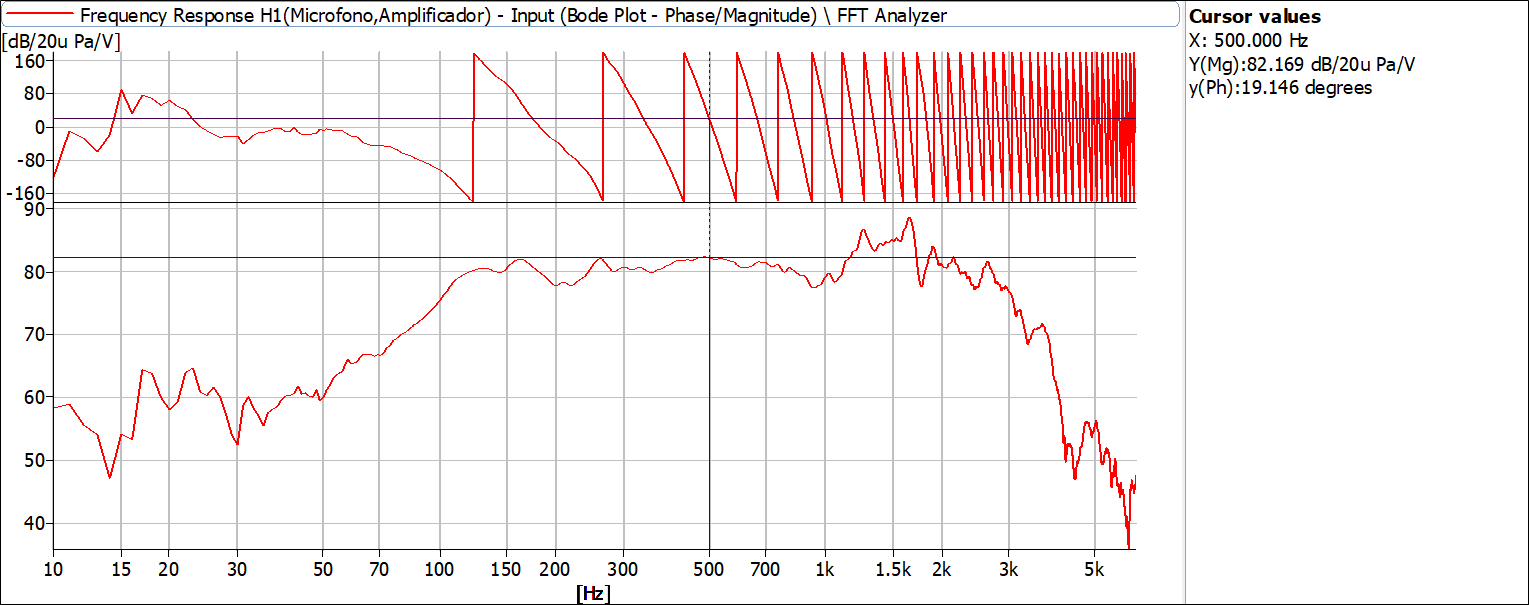
\includegraphics[width=\linewidth]{Picture1.png}
  \caption{Función de transferencia del woofer $H_1$ con el cursor situado en la frecuencia de \SI{500}{\Hz}.}
  \label{fig:Picture1}
\end{figure}

Se puede demostrar que ambos valores son equivalentes siguiendo los siguientes pasos:

\begin{align*}
   & \abs{H_1} = 20 \log \left( \frac{\abs{h_1}}{p _{\textnormal{ref}}} \right)                                                            \\
   & \rightarrow \quad \abs{h_1} = \num{20e-6}  \cdot 10 ^{\frac{82.2}{20}} = \qty{0.258}{\pascal }                                        \\
   & \rightarrow \quad \abs{H_1} = 20 \log \left( \frac{0.258}{1} \right) = \boxed{\SI{-11.8}{\dB} \text{ re. } \SI{1}{\pascal\per\volt} }
\end{align*}

\subsubsection{A partir de los resultados del laboratorio y tomando el valor de $H_1$ del apartado anterior, obtener la sensibilidad del \textit{woofer} usando estas tres expresiones:}
\begin{align} \label{eq:sens_1}
  S \left[ \SI{}{\dB\per\watt} \right] & = SPL_{\Delta} (r) + 20 \log \left( \frac{2.83}{V_{\Delta}} \right) + 20 \log \left( r \right)                                                                                                                       \\ \label{eq:sens_2}
  S \left[ \SI{}{\dB\per\watt} \right] & = H_1(r) \left[ \SI{}{\dB}\text{ re. }\SI{20}{\micro\pascal\per\volt} \right] + 20 \log \left( \frac{2.83}{1} \right) + 20 \log \left( r \right)                                                                     \\ \label{eq:sens_3}
  S \left[ \SI{}{\dB\per\watt} \right] & = H_1(r) \left[ \SI{}{\dB}\text{ re. }\SI{1}{\pascal\per\volt} \right] + 20 \log \left( \frac{2.83}{1} \right) + 20 \log \left( r \right) - \underbrace{20 \log \left( p _{\textnormal{ref}} \right)}_{\SI{94}{\dB}}
\end{align}

En primer lugar, se debe establecer el rango útil del altavoz a partir de la gráfica de la función de transferencia. En este caso se ha escogido que sea entre \qty{126.5}{\hertz } y \qty{2.563}{\kilo \hertz }.

Utilizando la \autoref{eq:sens_1} y los datos obtenidos de la , donde $SPL_{\Delta}$ es el nivel de presión sonora medido con el micrófono en la banda útil, $V_{\Delta}$ es la tensión de entrada en la banda útil y $r$ es la distancia entre el altavoz y el micrófono, se obtiene el valor de la sensibilidad $S$:

\[ S \left[ \unit{\dB\per\watt} \right] = SPL_{\Delta}(r) + 20 \log \left( \frac{2.83}{V_{\Delta}} + 20 \log \left( r \right)  \right) = 67.8 + 23.4 + 6 = \boxed{\qty{97.2}{\dB\per\watt}} \]

\begin{figure}[hbtp]
  \centering
  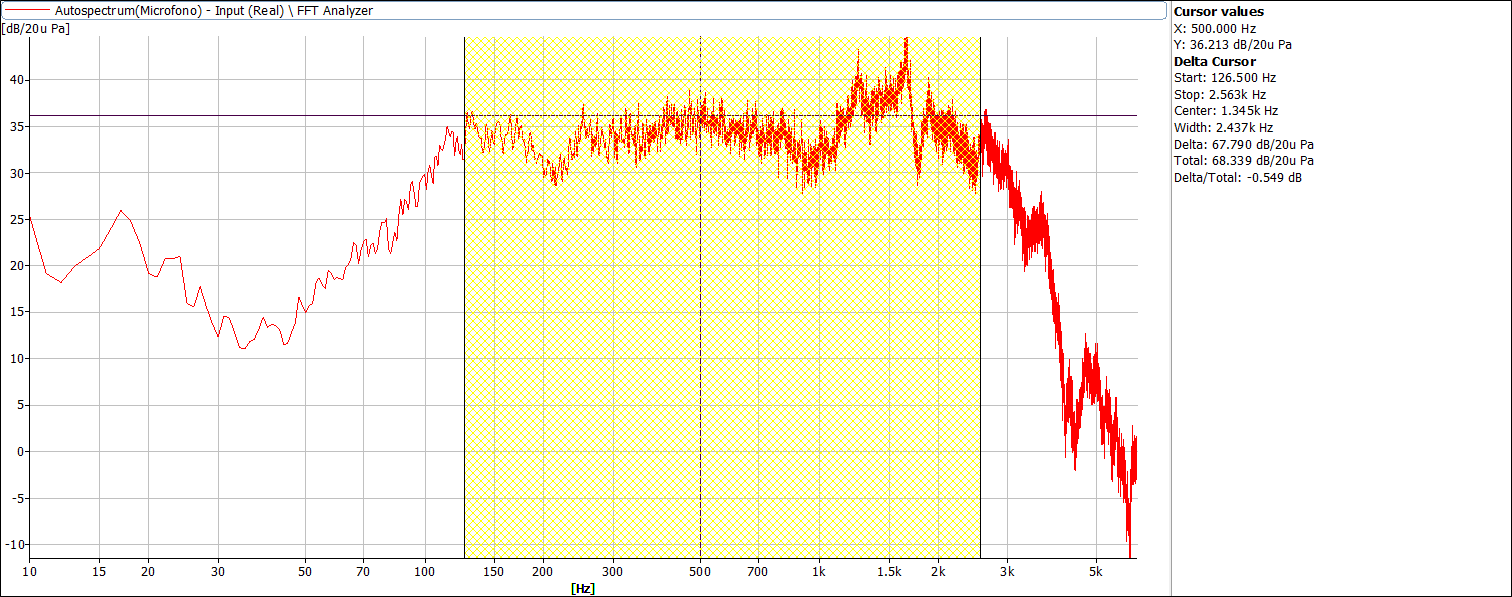
\includegraphics[width=\linewidth]{Picture2.png}
  \caption{Autoespectro de la señal captada por el micrófono.}
  \label{fig:Picture2}
\end{figure}

Ahora se procede a utilizar la \autoref{eq:sens_2}, donde $H_1(r)$ es el valor de la función de transferencia a lo largo del rango útil y a la distancia $r=\qty{2}{\metre }$. El valor medio de al función de transferencia se calcula en Excel y es:
\[ H_1(r=2) = \qty{81.8}{\dB} \text{ re. } \SI{20}{\micro\pascal\per\volt} \]

Y se obtiene el valor de $S$:
\begin{align*}
  S \left[ \unit{\dB\per\watt} \right] & = H_1(r=\qty{2}{\metre } + 20 \log \left( \frac{2.83}{1} \right) + 20 \log \left( \qty{2}{\metre } \right) \\
                                       & = 81.8 + 9 + 6 = \boxed{\qty{96.8}{\dB\per\watt}}                                                          \\
\end{align*}

Para utilizar la \autoref{eq:sens_3}, se debe cambiar el valor de presión de referencia en la propiedades de la gráfica. Una vez hecho esto, se calcula el valor medio de la función de transferencia en Excel, que da \qty{-12.2}{\dB}, y se obtiene el valor de $S$:
\[ S \left[ \unit{\dB\per\watt} \right] = -12.2 + 9 + 6 - 94 = \boxed{\qty{-91.2}{\dB\per\watt}} \]

Se aprecia que los tres resultados son coherentes entre sí, ya que las variaciones en el resultado son mínimas, y que por tanto las diferentes expresiones para calcular la sensibilidad son equivalentes.

\subsubsection{Calcular en Excel el valor $SPL_{\Delta}$ mediante las gráficas de la práctica.}

El procedimiento para calcular el valor de $SPL_{\Delta}$ en Excel es el siguiente:

\begin{itemize}
  \item Se copian los datos de la gráfica del nivel de presión sonora del micrófono y se pegan en una zona de la hoja de Excel.
  \item Se calcula una columna auxiliar de la presión cuadrática, corregida por el factor de correción de la ventana que utiliza Pulse. En este caso, el factor de corrección es $\sqrt{0.5}$. La fórmula de la $i$-ésima celda seguirá la siguiente fórmula:
        \[ p_i^2 = \frac{1}{\omega^2_{\text{rms}}} p^2 _{\textnormal{ref}} \cdot 10^{\frac{L_i}{10}} = \frac{1}{\left( \sqrt{1.5} \right)^2} \cdot \left( \num{20e-6} \right)^2 \cdot 10^{\frac{L_i}{10}} \]
  \item El nivel de presión sonora se calcula entonces como:
        \[ SPL_{\Delta} = 10 \log \left( \frac{\sum p_i^2}{p^2 _{\textnormal{ref}}} \right) = \qty{67.8}{\dB_{\text{SPL}}} \qquad \text{Siendo }p_i \text{ cada valor de presión medida en el rango útil} \]
\end{itemize}

Este valor coincide con el que muestra Pulse en la \autoref{fig:Picture2}.

\subsubsection{Mediante la fase de $H_1$ a \SI{600}{\Hz}, estimar la distancia $r$ a la que estaba el micrófono. Suponer que a esa frecuencia el altavoz tiene fase nula y la única fase captada es la fase acústica, $\varphi _a = -kr = \frac{-2\pi fr}{c}$.}

Colocando el cursor a \qty{600}{\hertz }, se obtiene un valor de fase de $\varphi _a = \ang{156.5}$ o $\varphi _a = \qty{2.73}{\radian }$. Sin embargo, se debe tener en cuenta que la fase está limitada en la gráfica a $\pm \qty{\pi}{\radian } $, por lo que si se haya por debajo de $\qty{-\pi}{\radian }$ se le sumará $\qty{2\pi}{\radian }$ y aparecerá representada como una fase positiva. Esto se manifiesta como una línea vertical de pendiente muy agresiva. A \qty{600}{\hertz } se han observado hasta 4 de esos saltos, por lo que la fase que se usará en la fórmula será $\varphi _a = 2.73 - 4 \cdot 2\pi = \qty{-22.4}{\radian } $. Asumiendo que la velocidad del sonido en el aire es de \qty{343}{\metre \per \second }, se obtiene la distancia:

\[ \varphi _a = \frac{-2\pi f r }{c} = \frac{-2\pi \cdot \qty{600}{\hertz } \cdot r}{343} = -22.4 \rightarrow r = \boxed{\qty{2.04}{\metre }} \]

\end{document}
